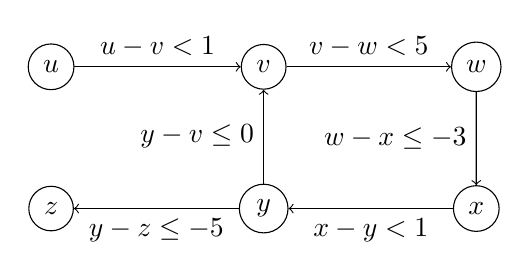
\begin{tikzpicture}[scale=0.9,state/.style={draw, circle, fill=none,text centered, text=black}]
    \node[state] (u) at (0, 2) {$u$};
    \node[state] (v) at (3, 2) {$v$};
    \node[state] (w) at (6, 2) {$w$};
    \node[state] (x) at (6, 0) {$x$};
    \node[state] (y) at (3, 0) {$y$};
    \node[state] (z) at (0, 0) {$z$};
    \draw [->] (u) -- node[anchor=south] {$ u-v < 1 $} (v);
    \draw [->] (v) -- node[anchor=south] {$ v-w < 5 $} (w);
    \draw [->] (w) -- node[anchor=east] {$ w-x \leq -3 $} (x);
    \draw [->] (x) -- node[anchor=north] {$ x-y < 1 $} (y);
    \draw [->] (y) -- node[anchor=north] {$ y-z \leq -5 $} (z);
    \draw [->] (y) -- node[anchor=east] {$ y-v \leq 0 $} (v);
\end{tikzpicture}
